\documentclass[10pt]{article}
\usepackage[letterpaper]{geometry}
\geometry{verbose,tmargin=1in,bmargin=1in,lmargin=1in,rmargin=1in}
\usepackage{setspace}
\usepackage{ragged2e}
\usepackage{color}
\usepackage{titlesec}
\usepackage{graphicx}
\usepackage{float}
\usepackage{mathtools}
\usepackage{amsmath}
\usepackage[font=small,labelfont=bf,labelsep=period]{caption}
\usepackage[english]{babel}
\usepackage{indentfirst}
\usepackage{array}
\usepackage{makecell}
\usepackage[usenames,dvipsnames]{xcolor}
\usepackage{multirow}
\usepackage{tabularx}
\usepackage{arydshln}
\usepackage{caption}
\usepackage{subcaption}
\usepackage{xfrac}
\usepackage{etoolbox}
\usepackage{cite}
\usepackage{url}
\usepackage{dcolumn}
\usepackage{hyperref}
\usepackage{courier}
\usepackage{esvect}
\usepackage{commath}
\usepackage{verbatim} % for block comments
\usepackage{enumitem}
\usepackage{hyperref} % for clickable table of contents
\usepackage{braket}
\usepackage{titlesec}
\usepackage{booktabs}
\usepackage{gensymb}
\usepackage{listings}
\usepackage{cancel}
\usepackage[mathscr]{euscript}
\lstset{
    frame=single,
    breaklines=true,
    postbreak=\raisebox{0ex}[0ex][0ex]{\ensuremath{\color{red}\hookrightarrow\space}}
}

% for circled numbers
\usepackage{tikz}
\newcommand*\circled[1]{\tikz[baseline=(char.base)]{
            \node[shape=circle,draw,inner sep=2pt] (char) {#1};}}

\newcommand{\beq}{\begin{equation}}
\newcommand{\eeq}{\end{equation}}
\newcommand{\beqa}{\begin{equation}\begin{aligned}}
\newcommand{\eeqa}{\end{aligned}\end{equation}}

\titleclass{\subsubsubsection}{straight}[\subsection]

% define new command for triple sub sections
\newcounter{subsubsubsection}[subsubsection]
\renewcommand\thesubsubsubsection{\thesubsubsection.\arabic{subsubsubsection}}
\renewcommand\theparagraph{\thesubsubsubsection.\arabic{paragraph}} % optional; useful if paragraphs are to be numbered

\titleformat{\subsubsubsection}
  {\normalfont\normalsize\bfseries}{\thesubsubsubsection}{1em}{}
\titlespacing*{\subsubsubsection}
{0pt}{3.25ex plus 1ex minus .2ex}{1.5ex plus .2ex}

\makeatletter
\renewcommand\paragraph{\@startsection{paragraph}{5}{\z@}%
  {3.25ex \@plus1ex \@minus.2ex}%
  {-1em}%
  {\normalfont\normalsize\bfseries}}
\renewcommand\subparagraph{\@startsection{subparagraph}{6}{\parindent}%
  {3.25ex \@plus1ex \@minus .2ex}%
  {-1em}%
  {\normalfont\normalsize\bfseries}}
\def\toclevel@subsubsubsection{4}
\def\toclevel@paragraph{5}
\def\toclevel@paragraph{6}
\def\l@subsubsubsection{\@dottedtocline{4}{7em}{4em}}
\def\l@paragraph{\@dottedtocline{5}{10em}{5em}}
\def\l@subparagraph{\@dottedtocline{6}{14em}{6em}}
\makeatother

\newcommand{\volume}{\mathop{\ooalign{\hfil$V$\hfil\cr\kern0.08em--\hfil\cr}}\nolimits}

\setcounter{secnumdepth}{4}
\setcounter{tocdepth}{4}
\begin{document}

\title{MATH 228b: HW3 ... 1c, 3bc, 4bc}
\author{April Novak}

\maketitle

\section{}

This problem solves the following differential equation:

\beq
\label{eq:prob}
-\nabla^2 u-k^2u=0
\eeq

With boundary conditions:

\beqa
\label{eq:BCs}
\hat{n}\cdot\nabla u=&0 & \textrm{ on } \Gamma_{wall}\\
\hat{n}\cdot\nabla u=&-iku & \textrm{ on } \Gamma_{out}\\
\hat{n}\cdot\nabla u=&2ik-iku & \textrm{ on } \Gamma_{in}\\
\eeqa

where the domain boundary is divided into three sections, where \(\Gamma=\Gamma_{wall}\cup\Gamma_{out}\cup\Gamma_{in}\). 

\subsection{(a)}

The weighted residual form is obtained by multiplying the governing equation by a weight function \(v\) and integrating over the domain, applying integration by parts when possible:

\beqa
-\int_{\Omega}v\nabla^2 u-\int_{\Omega}k^2uv=& 0\\
\int_{\Omega}\nabla u\cdot\nabla v-\int_{\Gamma}\hat{n}v\cdot\nabla u-\int_{\Omega}k^2uv=&0\\
\eeqa

Applying the boundary conditions:

\beq
\int_{\Omega}\nabla u\cdot\nabla v+\int_{\Gamma_{out}}viku-\int_{\Gamma_{in}}v(2ik-iku)-\int_{\Omega}k^2uv=0
\eeq

\(u\) is expanded in linear continuous polynomials over a series of elements \(K\) defined by a triangulation \(T_h\) such that:

\beq
u_h=\{u\in C^0(\Omega):u\rvert_K\in P_1(K)\forall K\in T_h, \textrm{for } \hat{n}\cdot\nabla u=0 \textrm{ on } \Gamma_{wall}, \hat{n}\cdot\nabla u=-iku \textrm{ on } \Gamma_{out}, \hat{n}\cdot\nabla u=2ik-iku \textrm{ on } \Gamma_{in}\}
\eeq

For a Galerkin approximation, \(v\) is chosen from the space \(V_h\), which is the same space as \(u_h\) except that \(V_h\) satisfy the homogeneous form of the essential boundary conditions (of which there are none in this problem):

\beq
V_h=\{v\in C^0(\Omega):v\rvert_K\in P_1(K)\forall K\in T_h\}
\eeq

The Galerkin finite element problem is therefore:

\beq
\int_{\Omega}\nabla u_h\cdot\nabla v_h+\int_{\Gamma_{out}}v_hiku_h+\int_{\Gamma_{in}}v_hiku_h-\int_{\Omega}k^2u_hv_h=\int_{\Gamma_{in}}v_h2ik
\eeq

\subsection{(b)}

\(u_h\) is represented as an expansion of basis functions described by the spaces given above:

\beq
u_h=\sum_{i=1}^{N}a_i\phi_i
\eeq

where \(N\) are the number of basis functions over the entire domain. Alternatively, this can be expressed in terms of the solution over each finite element:

\beq
u_h^e=\sum_{i=1}^{n_{en}}a_i\phi_i
\eeq

where \(n_{en}\) are the number of nodes per element and the \(e\) superscript indicates that the solution is only over a single element, with piecewise continuity between elements. Inserting these shape functions into the weak form above, where \(v_h\) is likewise expanded in the same set of basis functions as \(u_h\), but with expansion coefficients \(b\):

\beqa
\int_{\Omega}\nabla \left(\sum_{i=1}^{N}a_i\phi_i\right)\cdot\nabla \left(\sum_{j=1}^{N}b_j\phi_j\right)+\int_{\Gamma_{out}}\left(\sum_{j=1}^{N}b_j\phi_j\right)ik\left(\sum_{i=1}^{N}a_i\phi_i\right)+\int_{\Gamma_{in}}\left(\sum_{j=1}^{N}b_j\phi_j\right)ik\left(\sum_{i=1}^{N}a_i\phi_i\right)\\
-\int_{\Omega}k^2\left(\sum_{i=1}^{N}a_i\phi_i\right)\left(\sum_{j=1}^{N}b_j\phi_j\right)=\int_{\Gamma_{in}}\left(\sum_{j=1}^{N}b_j\phi_j\right)2ik
\eeqa

A simpler way of representing this weak form is to recognize that \(u_h\) and \(v_h\) can be represented as:

\beqa
u_h=&\textbf{N}\textbf{u}=\left\lbrack\phi_1, \phi_2, \cdots, \phi_N\right\rbrack\left\lbrack a_1, a_2, \cdots, a_N\right\rbrack^T\\
v_h=&\textbf{N}\textbf{v}=\left\lbrack\phi_1, \phi_2, \cdots, \phi_N\right\rbrack\left\lbrack b_1, b_2, \cdots, b_N\right\rbrack^T\\
\eeqa

The gradient of \(u_h\) is:

\beq
\nabla u_h=\textbf{B}\textbf{u}=\begin{bmatrix} 
\frac{\partial \phi_1}{\partial x} & \frac{\partial \phi_2}{\partial x} & \cdots & \frac{\partial \phi_N}{\partial x}\\
\frac{\partial \phi_1}{\partial y} & \frac{\partial \phi_2}{\partial y} & \cdots & \frac{\partial \phi_N}{\partial y}\\
\end{bmatrix}\textbf{u}
\eeq

The weak form can therefore equivalently be expressed as:

\beqa
\int_{\Omega}(\textbf{B}\textbf{u})\cdot(\textbf{B}\textbf{v})+\int_{\Gamma_{out}}(\textbf{N}\textbf{v})^Tik(\textbf{N}\textbf{u})+\int_{\Gamma_{in}}(\textbf{N}\textbf{v})^Tik(\textbf{N}\textbf{u})-\int_{\Omega}k^2(\textbf{N}\textbf{v})^T(\textbf{N}\textbf{u})=&\int_{\Gamma_{in}}(\textbf{N}\textbf{v})2ik\\
\int_{\Omega}(\textbf{B}\textbf{v})^T(\textbf{B}\textbf{u})+\int_{\Gamma_{out}}(\textbf{N}\textbf{v})^Tik(\textbf{N}\textbf{u})+\int_{\Gamma_{in}}(\textbf{N}\textbf{v})^Tik(\textbf{N}\textbf{u})-\int_{\Omega}k^2(\textbf{N}\textbf{v})^T(\textbf{N}\textbf{u})=&\int_{\Gamma_{in}}(\textbf{N}\textbf{v})^T2ik\\
\eeqa

Because \(\textbf{v}^T\) appears in every term, the above could be rearranged such that \(\textbf{v}^T\) multiplies an integrand, which equals zero, which would lead to the conclusion that the integrand itself must equal zero. In other words, \(\textbf{v}^T\) can essentially be canceled from every term.

\beqa
\int_{\Omega}\textbf{B}^T(\textbf{B}\textbf{u})+\int_{\Gamma_{out}}\textbf{N}^Tik(\textbf{N}\textbf{u})+\int_{\Gamma_{in}}\textbf{N}^Tik(\textbf{N}\textbf{u})-\int_{\Omega}k^2\textbf{N}^T(\textbf{N}\textbf{u})=&\int_{\Gamma_{in}}\textbf{N}^T2ik\\
\eeqa

To obtain a matrix equation in the form of that in the assignment, define:

\beqa
\label{eq:Matrices}
\textbf{K}=&\int_{\Omega}\textbf{B}^T\textbf{B}d\Omega\\
\textbf{M}=&\int_{\Omega}\textbf{N}^T\textbf{N}d\Omega\\
\textbf{B}_{in}=&\int_{\Gamma_{in}}\textbf{N}^T\textbf{N}d\Gamma\\
\textbf{B}_{out}=&\int_{\Gamma_{out}}\textbf{N}^T\textbf{N}d\Gamma\\
\textbf{b}_{in}=&\int_{\Gamma_{in}}\textbf{N}^Td\Gamma\\
\eeqa

Then, the overall matrix system is:

\beq
\left(\textbf{K}-k^2\textbf{M}+ik(\textbf{B}_{in}+\textbf{B}_{out})\right)\textbf{u}=2ik\textbf{b}_{in}
\eeq

Refer to the definitions of \textbf{N} and \textbf{B} to see these definitions in terms of the basis functions.

\subsection{(c)}

The transmitted intensity, when computed as a function of the finite element solution, is:

\beq
H(u_h)=\int_{\Gamma_{out}}|\textbf{N}\textbf{u}|^2
\eeq

where \(|(.)|\) is the complex absolute value of \((.)\). For vectors, the ``square'' is equivalent to a dot product, which by properties of the dot product can also be written in terms of transposes. By recognizing that the integral of \(\textbf{N}^T\textbf{N}\) is exactly that defined by \(\textbf{B}_{out}\) in Eq. \eqref{eq:Matrices}, the result that \(H(u_h\) can be expressed in terms of \(\textbf{u}\) has been shown.

\beqa
H(u_h)=&\int_{\Gamma_{out}}(\textbf{N}\textbf{u})\cdot(\textbf{N}\textbf{u})\\
H(u_h)=&\int_{\Gamma_{out}}(\textbf{N}\textbf{u})^T(\textbf{N}\textbf{u})\\
H(u_h)=&\int_{\Gamma_{out}}\textbf{u}^T\textbf{N}^T\textbf{N}\textbf{u}\\
H(u_h)=&\textbf{u}^T\textbf{B}_{out}\textbf{u}\\
\eeqa

\section{}

This problem solves the problem stated in Eq. \eqref{eq:prob} for boundary conditions given in Eq. \eqref{eq:BCs} for the rectangular domain given in the assignment.

\subsection{(a)}

The analytical solution to Eq. \eqref{eq:prob} with boundary conditions Eq. \eqref{eq:BCs} is only a function of \(x\), since the insulation boundary conditions along the top and bottom edges of the domain are symmetric. Hence, the PDE reduces to an ODE:

\beq
\frac{d^2u}{dx^2}+k^2u=0
\eeq

This common ODE has the following general solution:

\beqa
u(x)=&C_1sin(kx)+C_2cos(kx)\\
u(x)=&C_1\frac{1}{2i}\left(e^{ikx}-e^{-ikx}\right)+\frac{C_2}{2}\left(e^{ikx}+e^{-ikx}\right)\\
\eeqa

Apply the boundary condition on \(\Gamma_{in}\), where \(\hat{n}=\lbrack -1, 0\rbrack\) and \(x=0\):

\beqa
\lbrack -1, 0\rbrack\cdot(C_1kcos(kx)-C_2ksin(kx))=&2ik-ik(C_1sin(kx)+C_2cos(kx))\\
C_1=&-\frac{2ik-ikC_2}{k}\\
\eeqa

Applying the boundary condition on \(\Gamma_{out}\), where \(\hat{n}=\lbrack 1, 0\rbrack\) and \(x=5\):

\beqa
\lbrack 1, 0\rbrack\cdot(C_1kcos(5k)-C_2ksin(5k))=&-ik(C_1sin(5k)+C_2cos(5k))\\
C_1kcos(5k)-C_2ksin(5k)=&-ik(C_1sin(5k)+C_2cos(5k))\\
\eeqa

\beqa
u(x)=&-\frac{2-C_2}{2}\left(e^{ikx}-e^{-ikx}\right)+\frac{C_2}{2}\left(e^{ikx}+e^{-ikx}\right)\\
\eeqa

Applying the boundary condition on \(\Gamma_{out}\), where \(\hat{n}=\lbrack 1, 0\rbrack\) and \(x=5\):

\beqa
-\frac{2-C_2}{2}\left(e^{ikx}+e^{-ikx}\right)+\frac{C_2}{2}\left(e^{ikx}-e^{-ikx}\right)=&\frac{2-C_2}{2}\left(e^{ikx}-e^{-ikx}\right)-\frac{C_2}{2}\left(e^{ikx}+e^{-ikx}\right)\\
\frac{C_2}{2}\left\lbrack\left(e^{ikx}-e^{-ikx}+\left(e^{ikx}+e^{-ikx}\right)\right)\right\rbrack=&\frac{2-C_2}{2}\left\lbrack\left(e^{ikx}-e^{-ikx}\right)+\left(e^{ikx}+e^{-ikx}\right)\right\rbrack\\
\frac{C_2}{2}\left\lbrack e^{ikx}+e^{ikx}\right\rbrack=&\frac{2-C_2}{2}\left\lbrack e^{ikx}+e^{ikx}\right\rbrack\\
\frac{C_2}{2}=&\frac{2-C_2}{2}\\
C_2=&1\\
\eeqa

Then, \(C_1=-i\). Plugging these coefficients into the general solution gives the general solution for these boundaries.

\beqa
u(x)=&cos(kx)-isin(kx)\\
u(x)=&e^{-ikx}\\
\eeqa

\subsection{(b)}

The function {\tt waveguide\_edges} computes arrays of edges for the particular geometry for this question. By first finding all edges, the edges with both \(x\) coordinates equal to zero are on \(\Gamma_{in}\), while edges with both \(x\) coordinates equal to 5 are on \(\Gamma_{out}\), and edges with both \(y\) coordinates equal to 0 or 1 are on the \(\Gamma_{wall}\) boundary. The code developed for this section is shown in the Appendix.

\subsection{(c)}

This section computes the matrices given in Eq. \eqref{eq:Matrices} for a given mesh. To facilitate easier use of quadrature rules, all of the integrals in Eq. \eqref{eq:Matrices} are transformed to a master element, indicated by superscript \(e\) and variables of integration \(\xi\) and \(\eta\), as opposed to \(x\) and \(y\) in the physical domain. The boundary integrals are slightly more difficult to transform to the master domain. If the boundary corresponds to the bottom of the triangle in the master domain defined with corner points \((\xi=0,\eta=0), (\xi=1,\eta=0)\), then \(\eta=0\), and the integration is only with respect to \(\xi\) (and a normal, 1-D quadrature rule can be used). Likewise, if the boundary corresponds to the left edge of the master domain triangle defined by \((\xi=0,\eta=0), (\xi=0,\eta=1)\), then \(\xi=0\), and the integration is only with respect to \(\eta\). For elements with the hypotenuse of the master triangle on a boundary, the connectivity matrix is edited such that the edge along the boundary is the \(\xi\) edge (this is performed by simply shuffling the element row in the connectivity matrix by moving every number one position further to the right, and assigning the last number to the first column). Simpson's rule is used for integrating the boundary integrals, while the quadrature rule given in Question 4 is used for the area integrals. The code developed for this section is given in the Appendix. Also included in the Appendix is the code used for swapping location matrix (a.k.a. triangulation) indices.

\beqa
\label{eq:Matrices}
\textbf{K}^e=&\int_{\Omega^e}(\textbf{J}^{-1}\textbf{C})^T(\textbf{J}^{-1}\textbf{C})|\textbf{J}|d\eta d\xi\\
\textbf{M}^e=&\int_{\Omega^e}\textbf{N}^T\textbf{N}|\textbf{J}|d\eta d\xi\\
\textbf{B}_{in}^e=&\int_{\Gamma_{in}}\textbf{N}^T\textbf{N}d\Gamma\\
\textbf{B}_{out}^e=&\int_{\Gamma_{out}}\textbf{N}^T\textbf{N}d\Gamma\\
\textbf{b}_{in}^e=&\int_{\Gamma_{in}}\textbf{N}^Td\Gamma\\
\eeqa

where \textbf{J} and \textbf{C} are defined as:

\beqa
\textbf{J}=&\begin{bmatrix}dx/d\xi & dx/d\eta\\ dy/d\xi & dy/d\eta\end{bmatrix}\\
\textbf{C}=&\begin{bmatrix}
\frac{\partial\psi_1}{d\xi} & \frac{\partial\psi_2}{d\xi} & \cdots & \frac{\partial\psi_{n_en}}{d\xi}\\
\frac{\partial\psi_1}{d\eta} & \frac{\partial\psi_2}{d\eta} & \cdots & \frac{\partial\psi_{n_en}}{d\eta}\\
\end{bmatrix}\\ 
\eeqa

\subsection{(d)}

Finally, {\tt femhelmholtz.m} is used to solve the given domain for successively finer and finer meshes to determine the rate of convergence. A short script was developed to show the convergence, and is included in the Appendix. The rate of convergence is estimated as {\tt rate=log2(errors(end-1))-log2(errors(end))}, and is approximately 1.9854. This is to be expected, since the rate of convergence of the finite element method, for sufficiently smooth solutions (which is the case here, since cosines and sines are infinitely differentiable), is only dependent on the polynomial order and an unknown constant. Hence, from the previous assignment, a convergence rate of 2 is obtained for linear elements (and a convergence rate of 3 would be obtained for quadratic elements).

\begin{figure}[H]
\centering
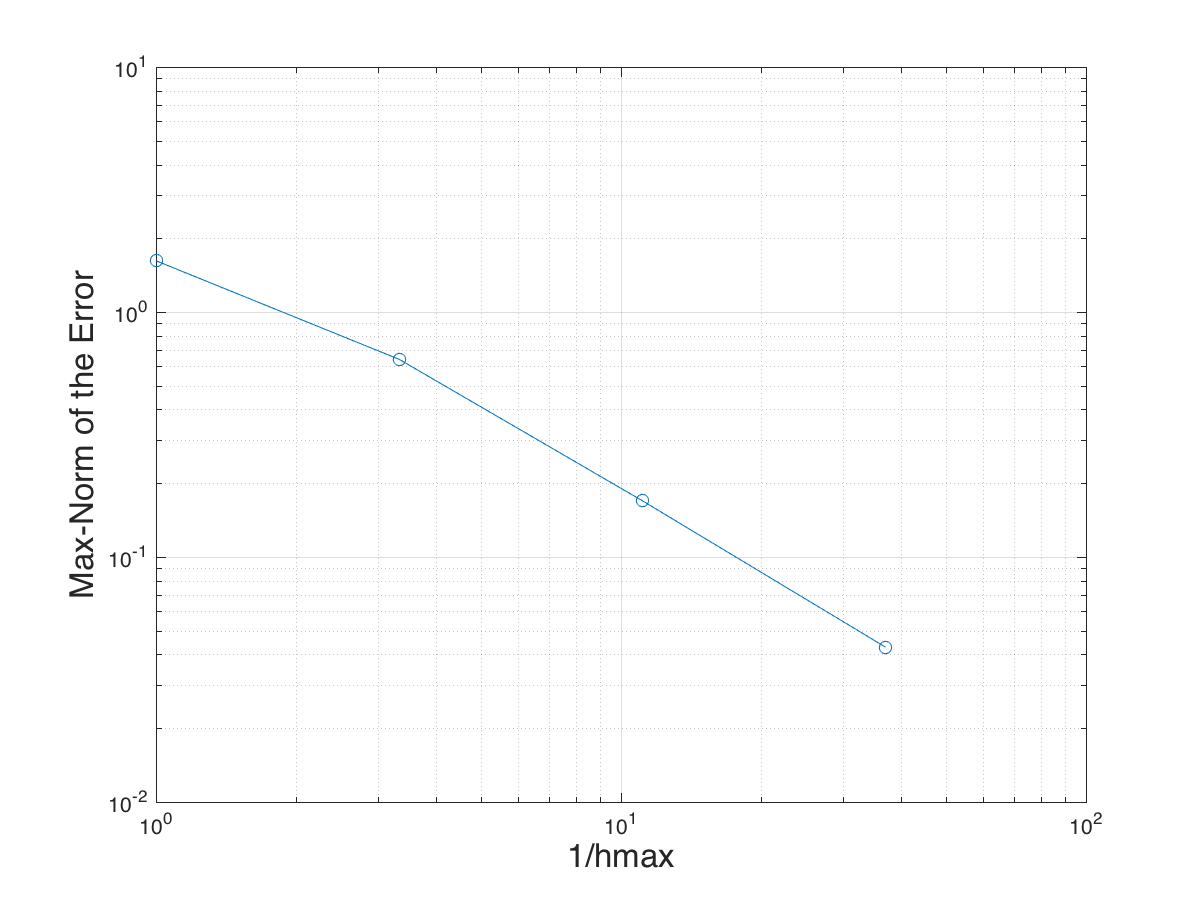
\includegraphics[width=0.6\textwidth]{error.png}
\caption{Max norm of the error between the analytic and finite element method solutions.}
\label{fig:1}
\end{figure}





\section{} % QUESTION 3

{\tt pmesh.m} (the one developed by the Professor, since I got points off from HW 1 for my {\tt pmesh}) is used to generate a mesh of the domain given in the assignment. 

\subsection{(a)}

Fig. \ref{fig:q3mesh} shows the mesh generated for this domain.

\begin{figure}[H]
\centering
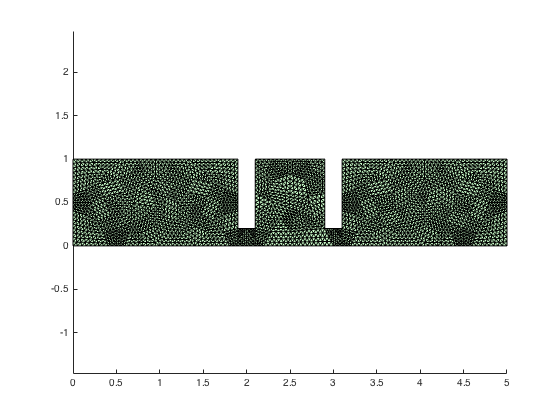
\includegraphics[width=0.8\textwidth]{mesh_q3.png}
\caption{Mesh generated for the provided domain using {\tt pmesh}.}
\label{fig:q3mesh}
\end{figure}

\subsection{(b)}





% QUESTION 4
\section{}

This problem extends the {\tt fempoi.m} solver developed in the previous homework for quadratic triangular elements. All triangle are assumed to have straight edges. 

\subsection{(a)}

A mesh developed for linear basis functions can easily be extended to a mesh for quadratic basis functions by simply adding three additional nodes per triangle, one at the midpoint of each side. The additional points are added to the original mesh by looping over the triangles and adding the midpoints of every side, and the calling {\tt unique} to remove (roughly) half of these points which are shared by two triangles. Then, a loop is created that loops over all of the original triangles and re-computes these midpoints and then searches through the (original + new) list of points to determine the row number of that point. Then, the new triangulation is defined such that the corners of the original triangle fill the 1, 3, and 5 entries of the new triangulation, with the 2, 4, and 6 entries given as the row number of the midpoint along the corresponding edge.

To determine which of the original nodes (in {\tt p}) are on the boundary, {\tt boundary\_nodes} is used. Then, to determine which of the new nodes are on the boundary, if two nodes in the same triangle are both on the boundary, then the midpoint node on the edge between those two corner points is in most situations also on the boundary. However, in some cases, when all three corner nodes of a triangle are on the boundary, then at least one of the midpoint nodes is actually not in the boundary. So, a loop over all of the rows and columns in the triangulation is used to determine if a point appears more than once in the triangulation - if so, it is not actually on the boundary. In this way, the boundary nodes, consisting of the original boundary nodes and the new boundary nodes, is created. The code developed for this section is shown in the Appendix.

\subsection{(b)}

This problem solves the Poisson equation from the previous homework using quadratic Lagrange elements. The equation to be solved is:

\beqa
-\nabla^2u(x,y)=1\\
u\rvert_{\Gamma_d}=0,\quad \hat{n}\cdot\nabla u\rvert_{\Gamma_t}=0\\
\eeqa

where \(\Gamma_d\) indicates the Dirichlet portion of the boundary and \(\Gamma_t\) the Neumann portion of the boundary, and \(\Gamma_d\cup\Gamma_t=\Gamma\). The weighted residual form is obtained by multiplying the above by a weight function \(v\):

\beq
-\int_\Omega \nabla^2u(x,y)v(x,y)d\Omega=\int_\Omega v(x,y)d\Omega
\eeq

The weak form is obtained by integrating by parts:

\beq
\int_\Omega \nabla u(x,y)\cdot\nabla v(x,y)d\Omega-\int_\Gamma\hat{n}\cdot\nabla u(x,y)v(x,y)d\Gamma=\int_\Omega v(x,y)d\Omega
\eeq

Homogeneous Neumann conditions allow the boundary term above to simply be dropped, since \(\hat{n}\cdot\nabla u(x,y)=0\) on \(\Gamma_t\) and the weight function \(v(x,y)\) satisfies the homogeneous form of the essential boundary conditions on the essential boundaries such that \(v(x,y)=0\) for all remaining parts of the boundary (since \(\Gamma_d\cap\Gamma_t=\emptyset\)). After removing this term, the following represents the weak form for the problem, where processing of the global stiffness matrix and global load vector are required to ensure that the solution obtains the specified values on the Dirichlet boundaries.

\beq
\int_\Omega \nabla u(x,y)\cdot\nabla v(x,y)d\Omega=\int_\Omega v(x,y)d\Omega
\eeq

\(u\) is approximated as \(u_h\) by expanding it in a series of basis functions \(\psi\):

\beq
u_h=\sum_{i=1}^{N}a_j\psi_j(x,y)
\eeq

where \(N\) is the total number of basis functions, which for Lagrange elements is equivalent to the number of nodes in the domain. Instead of defining basis functions that exist over the entire domain, to improve the sparsity of the matrices involved, expand \(u_h\) in \(n_{en}\) basis functions over each finite element, where \(n_{en}\) are the number of nodes per element. 

\beq
u_h^k=\sum_{i=1}^{n_{en}}a_j\psi_j(x,y)=\textbf{N}\textbf{u}
\eeq

The right-hand side can be represented as two vectors, one containing the shape functions, and the other containing the expansion coefficients. 

\beq
\textbf{N}=\begin{bmatrix} \psi_1(x,y) & \psi_2(x,y) & \cdots & \psi_{n_{en}}\end{bmatrix}
\eeq

\beq
\textbf{u}=\begin{bmatrix} a_1 & a_2 & \cdots & a_{n_{en}}\end{bmatrix}^T
\eeq

Likewise, the weight function \(v\) can also be expanded in the same manner, but with different expansion coefficients \textbf{b}. The gradient of \(u_h\) is defined as:

\beq
\nabla u_h=\frac{\partial u_h}{\partial x}\hat{x}+\frac{\partial u_h}{\partial y}\hat{y}=\textbf{B}\textbf{u}
\eeq

where \textbf{B} is a deformation matrix that acts on the solution \textbf{u} to produce the effect of the gradient. 

\beq
\textbf{B}=\begin{bmatrix}
\frac{\partial\psi_1}{dx} & \frac{\partial\psi_2}{dx} & \cdots & \frac{\partial\psi_{n_en}}{dx}\\
\frac{\partial\psi_1}{dy} & \frac{\partial\psi_2}{dy} & \cdots & \frac{\partial\psi_{n_en}}{dy}\\
\end{bmatrix}
\eeq

Then, noting that the dot product of two vectors can be written as \(\textbf{a}\cdot\textbf{b}=\textbf{a}^T\textbf{b}\), the weak form becomes:

\beqa
\int_\Omega (\textbf{B}\textbf{u})^T(\textbf{B}\textbf{v})d\Omega=&\int_\Omega \textbf{N}\textbf{v}d\Omega\\
\int_\Omega \textbf{B}^T\textbf{u}^T(\textbf{B}\textbf{v})d\Omega=&\int_\Omega \textbf{N}\textbf{v}d\Omega\\
\int_\Omega \textbf{B}^T\textbf{u}\textbf{B}d\Omega=&\int_\Omega \textbf{N}d\Omega\\
\eeqa

where \textbf{v} has essentially been cancelled from every term (the above could be rearranged such that \textbf{v} acts on an integrand, where the entire term equals zero such that the integrand must therefore equal zero). The above is essentially equivalent to the 1-D form, where \textbf{B} would reduce to \(d\psi_i/dx\) and \textbf{N} to \(\psi_i\). The elemental stiffness matrix and elemental load vector are:

\beq
\label{eq:20}
\textbf{A}^k=\int_{\Omega_k} \textbf{B}^T\textbf{B}d\Omega
\eeq

\beq
\label{eq:21}
\textbf{F}^k=\int_{\Omega_k} \textbf{N}d\Omega
\eeq

In order to apply over an individual element, the shape functions that appear in \textbf{B} and \textbf{N} must be the shape functions over that particular element. This can be achieved either by determining the shape functions over each element in the physical domain (in which case the shape functions are different for every element) or by using isoparametric elements that are mapped from a master domain, where the integrals above are always the same, and then modify the above terms with a Jacobian of the transformation. Therefore, a key difference between {\tt fempoi2} and {\tt fempoi} is the selection of these boundary conditions. To determine these shape functions over the master element, a quadratic shape function has the form \(\psi(x)=a+bx+cy+dx^2+ey^2+fxy\). If these shape functions are determined individually for each element, they would be determined by solving the following system for the six different right-hand sides shown below to give the coefficients \(a, b, c, d, e, f\) for each of the six shape functions (assuming quadratic triangular elements for this problem):

\beq
\begin{bmatrix} 1 & x_1 & y_1 & x_1^2 & y_1^2 & x_1y_1\\1 & x_2 & y_2 & x_2^2 & y_2^2 & x_2y_2\\1 & x_3 & y_3 & x_3^2 & y_3^2 & x_3y_3\\1 & x_4 & y_4 & x_4^2 & y_4^2 & x_4y_4\\1 & x_5 & y_5 & x_5^2 & y_5^2 & x_5y_5\\1 & x_6 & y_6 & x_6^2 & y_6^2 & x_6y_6\end{bmatrix}
\begin{bmatrix}a\\ b\\ c\\d\\e\\f\end{bmatrix}=\begin{bmatrix}1\\ 0\\ 0\\0\\0\\0\end{bmatrix};\ \begin{bmatrix}0\\ 1\\ 0\\0\\0\\0\end{bmatrix};\ \begin{bmatrix}0\\ 0\\ 1\\0\\0\\0\end{bmatrix};\ \begin{bmatrix}0\\ 0\\ 0\\1\\0\\0\end{bmatrix};\ \begin{bmatrix}0\\ 0\\ 0\\0\\1\\0\end{bmatrix};\ \begin{bmatrix}0\\ 0\\ 0\\0\\0\\1\end{bmatrix}
\eeq

where \(x_i, y_i\) is the \(i\) coordinate of the triangle, for \(i=1, 2, 3, 4, 5, 6\). Performing this for every triangle individually is tedious, and likewise determining the appropriate bounds of integration for each triangle is problematic and difficult when only the coordinate points are known. To overcome this, a mapping is performed from a master triangle with corners at \((0,0), (1,0), (0,1)\) and midpoints at \((0.5,0), (0.5,0.5), (0,0.5)\) in a coordinate system defined in terms of variables \(\xi\) and \(\eta\). The shape functions in this master domain will therefore be the same over each element in the physical domain, and the only thing that differs for each element is the Jacobian of the transformation. With \((x_1=0, y_1=0), (x_2=0.5, y_2=0), (x_3=1,y_3=0), (x_4=0.5,y_4=0.5), (x_5=0,y_5=1), (x_6=0,y_6=0.5)\), the shape functions in the master domain are:

\beqa
\psi_1(\xi,\eta)=&1-3\xi-3\eta+2\xi^2+2\eta^2+4\xi\eta\\
\psi_2(\xi,\eta)=&4\xi-4\xi^2-4\xi\eta\\
\psi_3(\xi,\eta)=&-\xi+2\xi^2\\
\psi_4(\xi,\eta)=&4\xi\eta\\
\psi_5(\xi,\eta)=&-\eta+2\eta^2\\
\psi_6(\xi,\eta)=&4\eta-4\eta^2-4\xi\eta\\
\eeqa

The mapping from the master to physical domain is performed using an isoparametric mapping that relates the physical coordinates \((X_i,Y_i)\) to the master domain coordinates \((\xi,\eta)\)

\beqa
x(\xi,\eta)=&\sum_{i=1}^{n_{en}}X_i\psi_i(\xi,\eta)\\
y(\xi,\eta)=&\sum_{i=1}^{n_{en}}Y_i\psi_i(\xi,\eta)\\
\eeqa

To transform the integrals appearing in Eq. \eqref{eq:20} and \eqref{eq:21} to integrals over the master domain requires the use of the derivatives with respect to \(\xi\) and \(\eta\), rather than with respect to \(x\) and \(y\). The domain of integration changes according to:

\beqa
d\vv{x}=&\textbf{D}d\vv{\xi}\\
\begin{bmatrix}dx\\dy\end{bmatrix}=&
\begin{bmatrix}dx/d\xi & dx/d\eta\\ dy/d\xi & dy/d\eta\end{bmatrix}
\begin{bmatrix}d\xi\\d\eta\end{bmatrix}
\eeqa

where \textbf{D} is the transformation matrix that describes how the coordinate transformation is performed. The derivatives appearing in \textbf{D} are computed based on the definitions of the isoparametric mapping:

\beqa
\frac{dx(\xi,\eta)}{d\xi}=&\sum_{i=1}^{n_{en}}X_i\frac{d\psi_i(\xi,\eta)}{d\xi}\\
\frac{dx(\xi,\eta)}{d\eta}=&\sum_{i=1}^{n_{en}}X_i\frac{d\psi_i(\xi,\eta)}{d\eta}\\
\frac{dy(\xi,\eta)}{d\xi}=&\sum_{i=1}^{n_{en}}Y_i\frac{d\psi_i(\xi,\eta)}{d\xi}\\
\frac{dy(\xi,\eta)}{d\eta}=&\sum_{i=1}^{n_{en}}Y_i\frac{d\psi_i(\xi,\eta)}{d\eta}\\
\eeqa

With these definitions, the local stiffness matrix and local load vector transform to integrals over \(\xi, \eta\):

\beq
\label{eq:20}
\textbf{A}^k=\int_{0}^{1} \int_{0}^{1-\xi}(\textbf{D}^{-1}\textbf{C})^T(\textbf{D}^{-1}\textbf{C})|\textbf{D}| d\eta d\xi
\eeq

\beq
\label{eq:21}
\textbf{F}^k=\int_{0}^{1} \int_{0}^{1-\xi}\textbf{N}|\textbf{D}| d\eta d\xi
\eeq

where \textbf{C} is the same as \textbf{B}, except that derivatives are taken with respect to \(\xi\) and \(\eta\) instead of \(x\) and \(y\):

\beq
\textbf{C}=\begin{bmatrix}
\frac{\partial\psi_1}{d\xi} & \frac{\partial\psi_2}{d\xi} & \cdots & \frac{\partial\psi_{n_en}}{d\xi}\\
\frac{\partial\psi_1}{d\eta} & \frac{\partial\psi_2}{d\eta} & \cdots & \frac{\partial\psi_{n_en}}{d\eta}\\
\end{bmatrix}
\eeq

Note that the integrals in Eq. \eqref{eq:20} and \eqref{eq:21} are no longer over the domain of an element in the physical domain - they are over a triangle in the master domain. To allow easy calculation of these integrals without the need to use symbolic integration or the need to hard-code in the integrals given that all of the shape functions are linear in \(x\) and \(y\) (to permit faster extension to higher-order elements), quadrature rules are used to numerically evaluate the integrals above. A second motivation to using the transformation to the master domain is the ability to use the same quadrature rule over every element. Quadrature rules for the standard triangle defined with corners at \((0,0), (1,0), (0,1)\) are attempting to determine the weights \(w_i\) and quadrature points \(\xi_i,\eta_i\) so that the following summation is as accurate as possible for a polynomial of some given order:

\beq
\int_{0}^{1} \int_{0}^{1-\xi}f(\xi,\eta)d\eta d\xi\approx\sum_{i=1}^{n_{qp}}w_if(\xi_i,\eta_i)
\eeq

For \(n_{qp}=3\), the following three-point rule exactly integrates quadratic integrands over the master domain with corners at \((\xi_1=0,\eta_1=0), (\xi_2=1,\eta_2=0), (\xi_3=0,\eta_3=1)\).

\beqa
w=&\begin{bmatrix}1/3& 1/3& 1/3\end{bmatrix}\\
(\xi_i,\eta_i)=&\begin{bmatrix}\sum_{j=1}^3\left(\frac{\xi_j}{6}+\frac{\xi_1}{2}\right) & \sum_{j=1}^3\left(\frac{\eta_j}{6}+\frac{\eta_1}{2}\right)\\
\sum_{j=1}^3\left(\frac{\xi_j}{6}+\frac{\xi_2}{2}\right) & \sum_{j=1}^3\left(\frac{\eta_j}{6}+\frac{\eta_2}{2}\right)\\
\sum_{j=1}^3\left(\frac{\xi_j}{6}+\frac{\xi_3}{2}\right) & \sum_{j=1}^3\left(\frac{\eta_j}{6}+\frac{\eta_3}{2}\right)
 \end{bmatrix}\\
=&\begin{bmatrix}\frac{1}{6}\left(\xi_1+\xi_2+\xi_3\right) & \frac{1}{6}\left(\eta_1+\eta_2+\eta_3\right)\\
\frac{1}{6}\left(\xi_1+\xi_2+\xi_3\right)+\frac{3}{2} & \frac{1}{6}\left(\eta_1+\eta_2+\eta_3\right)\\
\frac{1}{6}\left(\xi_1+\xi_2+\xi_3\right) & \frac{1}{6}\left(\eta_1+\eta_2+\eta_3\right)+\frac{3}{2}
 \end{bmatrix}\\
 =&\begin{bmatrix}1/6 & 1/6\\
1/6+3/2 & 1/6\\
1/6 & 1/6+3/2
 \end{bmatrix}
\eeqa

Then, the quadrature-integrated integral is multiplied by the area of the triangle, which is \(1/2\) for the master triangle. The elemental stiffness matrix and elemental load vector are computed for each individual element. They are then assembled in the global matrix according to the connectivity matrix, which is conveniently provided as the triangulation returned by the {\tt delaunay} function. For example, with the following triangulation for a domain where each element has four nodes, the connectivity matrix, also called the location matrix (LM), would be:

\begin{equation}
\textbf{LM}=\begin{bmatrix}
1 & 2 & 5 & 4\\
2 & 3 & 6 & 5\\
4 & 5 & 8 & 7\\
5 & 6 & 9 & 8\\
\end{bmatrix}
\end{equation}

where the local nodes are numbered in a counterclockwise manner beginning from the bottom left node. Then, for example, the second row in the global stiffness matrix would be assembled as:

\begin{equation}
\textbf{K}(2,:)=\begin{bmatrix}
k_{2,1}^{e=1}, & k_{2,2}^{e=1}+k_{1,1}^{e=2}, & k_{1,2}^{e=2}, & k_{2,4}^{e=1}, & k_{1,4}^{e=2}+k_{2,3}^{e=1}, & k_{1,3}^{e=2}, & 0, & 0, & 0\\
\end{bmatrix}
\end{equation}

Then, similar to the discussion in Problem 2, instead of solving \(\textbf{A}\textbf{u}=\textbf{f}\) using the full matrices above, the following system must be solved:

\beq
A_{uu}u_u=f_u-A_{uk}x_k
\eeq


\section{Appendix}
\subsection{Question 2}
\subsubsection{Part (b) - {\tt waveguide\_edges.m}}
\lstinputlisting[language=Matlab]{waveguide_edges.m}
\subsubsection{Part (c) - {\tt femhelmholtz.m}}
\lstinputlisting[language=Matlab]{femhelmholtz.m}
\subsubsection{Part (c) - {\tt changeLM.m}}
\lstinputlisting[language=Matlab]{changeLM.m}
\subsubsection{Part (d) - {\tt convergence\_helmholtz.m}}
\lstinputlisting[language=Matlab]{convergence_helmholtz.m}
\subsection{Question 4}
\subsubsection{Part (a) - {\tt p2mesh.m}}
\lstinputlisting[language=Matlab]{p2mesh.m}

\end{document}
